% Standalone XeLaTeX source. Uses standard commands and distributed packages.
% Source problem: public/notes/物工/問題/2015ap_exam.pdf, PDF pages 11–12.
\documentclass[11pt,a4paper]{article}
\usepackage[margin=24mm]{geometry}
\usepackage{fontspec}
\usepackage{xeCJK}
\setCJKmainfont{HaranoAjiMincho-Regular.otf}
\setCJKsansfont{HaranoAjiGothic-Medium.otf}
\usepackage{amsmath,amssymb}
\usepackage{tikz}
\usetikzlibrary{arrows.meta}
\setlength{\parindent}{1em}
\setlength{\parskip}{0.35em}
\renewcommand{\figurename}{図}
\title{物理工学専攻 院試解答集 ver2\\2015年 物理学II 第4問}
\author{政岡凜太郎}
\date{}
\begin{document}
\maketitle

\section*{[1.1] 放物線バンドの状態密度}
エネルギーが$\epsilon>0$以下の状態は$\boldsymbol k$空間で楕円体の内部にある。その半軸は$k_i=\sqrt{2m_i\epsilon}/\hbar$である。スピン自由度を数えず、$\boldsymbol k$空間で1状態が占める体積を$(2\pi)^3$とすると、単位実空間体積当たりの状態数は
\begin{equation}
  n(\epsilon)=\frac{1}{(2\pi)^3}\frac{4\pi}{3}
  \prod_{i=1}^{3}\frac{\sqrt{2m_i\epsilon}}{\hbar}
  =\frac{(2\epsilon)^{3/2}\sqrt{m_1m_2m_3}}{6\pi^2\hbar^3}.
\end{equation}
これを$\epsilon$で微分して
\begin{equation}
  \boxed{\rho_{3\mathrm D}(\epsilon)=
  \frac{\sqrt{2m_1m_2m_3\epsilon}}{2\pi^2\hbar^3}\quad(\epsilon\ge0),}
\end{equation}
負のエネルギーでは$\rho_{3\mathrm D}=0$である。状態密度はバンド端から$\sqrt\epsilon$に比例して増加する。

\section*{[1.2] 波数の時間発展}
速度成分は$v_x=\hbar k_x/m_1$、$v_y=\hbar k_y/m_2$、$v_z=\hbar k_z/m_3$である。電子の符号$-e$と$\boldsymbol B=(0,0,B)$から
\begin{equation}
  \dot k_x=-\frac{eB}{m_2}k_y,\qquad
  \dot k_y=\frac{eB}{m_1}k_x,\qquad
  \dot k_z=0.
\end{equation}
従って$\ddot k_x=-(eB)^2k_x/(m_1m_2)$であり、正の角周波数は
\begin{equation}
  \boxed{\omega_c=\frac{eB}{\sqrt{m_1m_2}}}.
\end{equation}
初期条件と設問の$k_x$の形より
\begin{equation}
  \boxed{k_x(t)=k_{0x}\cos(\omega_ct),\quad
  k_y(t)=\sqrt{\frac{m_2}{m_1}}k_{0x}\sin(\omega_ct),\quad
  k_z(t)=k_{0z}.}
\end{equation}

\section*{[1.3] 波数軌道}
消去すると
\begin{equation}
  \frac{k_x^2}{k_{0x}^2}+
  \frac{k_y^2}{(\sqrt{m_2/m_1}\,k_{0x})^2}=1.
\end{equation}
したがって$k_x$–$k_y$平面では楕円を描く。$t=0$で$(k_x,k_y)=(k_{0x},0)$にあり、$\dot k_y(0)>0$なので、時間とともに上向きに進む。


\begin{figure}[htbp]
\centering
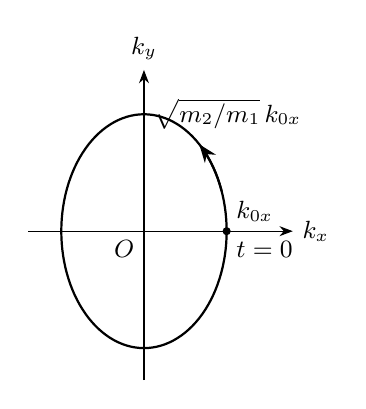
\begin{tikzpicture}[>=Stealth,font=\small,scale=1.05]
 \pgfmathsetmacro{\kb}{sqrt(2)}
 \draw[->] (-1.4,0)--(1.8,0) node[right] {$k_x$};
 \draw[->] (0,-1.8)--(0,1.95) node[above] {$k_y$};
 \draw[thick] plot[domain=0:360,samples=121] ({cos(\x)},{\kb*sin(\x)});
 \draw[->,thick] plot[domain=20:48,samples=16] ({cos(\x)},{\kb*sin(\x)});
 \fill (1,0) circle (1.4pt) node[below right] {$t=0$};
 \draw (1,-0.06)--(1,0.06); \node[above right] at (1,0) {$k_{0x}$};
 \draw (-0.06,\kb)--(0.06,\kb); \node[right] at (0,\kb) {$\sqrt{m_2/m_1}\,k_{0x}$};
 \node[below left] at (0,0) {$O$};
\end{tikzpicture}
\caption{放物線バンドの波数軌道。$m_2=2m_1$の例を描いた。軸上のラベルは一般の半軸長であり、矢印は時間の増加方向を示す。}
\label{fig:parabolic-k}
\end{figure}

\section*{[1.4] 実空間の軌道}
群速度を積分し、$\boldsymbol r(0)=0$を使うと
\begin{align}
  x(t)&=\frac{\hbar k_{0x}}{m_1\omega_c}\sin(\omega_ct),\\
  y(t)&=\frac{\hbar k_{0x}}{\sqrt{m_1m_2}\,\omega_c}
       [1-\cos(\omega_ct)],\\
  z(t)&=\frac{\hbar k_{0z}}{m_3}t.
\end{align}
$xy$平面への射影は中心が$y=\hbar k_{0x}/(\sqrt{m_1m_2}\,\omega_c)$にある楕円である。$t=0$では原点から$x$正方向へ進む。$z$は一定速度で増えるので、三次元軌道はこの楕円を射影にもつらせんである。


\begin{figure}[htbp]
\centering
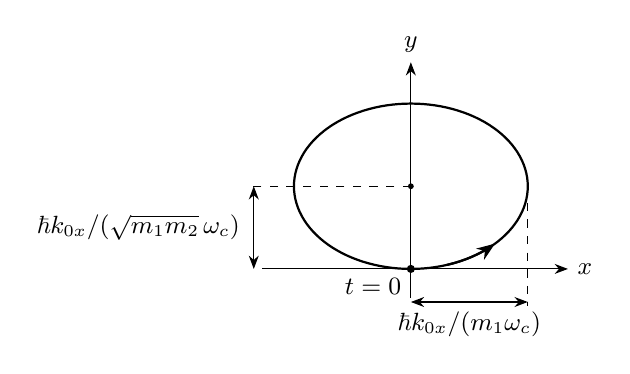
\begin{tikzpicture}[>=Stealth,font=\small,scale=1.05]
 \pgfmathsetmacro{\rx}{sqrt(2)}
 \draw[->] (-1.8,0)--(1.9,0) node[right] {$x$};
 \draw[->] (0,-0.35)--(0,2.5) node[above] {$y$};
 \draw[thick] plot[domain=0:360,samples=121] ({\rx*sin(\x)},{1-cos(\x)});
 \draw[->,thick] plot[domain=18:46,samples=16] ({\rx*sin(\x)},{1-cos(\x)});
 \fill (0,0) circle (1.4pt) node[below left] {$t=0$};
 \fill (0,1) circle (1pt);
 \draw[dashed] (\rx,1)--(\rx,-0.45);
 \draw[<->] (0,-0.4)--(\rx,-0.4)
   node[midway,below] {$\hbar k_{0x}/(m_1\omega_c)$};
 \draw[dashed] (0,1)--(-2.0,1);
 \draw[<->] (-1.9,0)--(-1.9,1);
 \node[left] at (-1.95,0.5) {$\hbar k_{0x}/(\sqrt{m_1m_2}\,\omega_c)$};
\end{tikzpicture}
\caption{放物線バンドの実空間軌道の$xy$射影。図\ref{fig:parabolic-k}と同じ$m_2=2m_1$の例。初期位置は原点で、矢印は時間の増加方向を示す。}
\label{fig:parabolic-r}
\end{figure}


\section*{[2.1] 線形バンドの状態密度}
2次元では状態密度は$\boldsymbol k$空間の面積で数える。エネルギーの絶対値が$|\epsilon|$以下の状態の波数半径は$k=|\epsilon|/\gamma$であり、1枝当たりの単位面積当たり状態数は
\begin{equation}
  n(\epsilon)=\frac{\pi k^2}{(2\pi)^2}
  =\frac{\epsilon^2}{4\pi\gamma^2}.
\end{equation}
正負どちらの枝についても$|\epsilon|$で微分した状態密度は
\begin{equation}
  \boxed{\rho_{2\mathrm D}(\epsilon)=\frac{|\epsilon|}{2\pi\gamma^2}.}
\end{equation}
よって$\epsilon=0$でゼロとなり、正負のエネルギーに対してV字形に増加する。

\begin{figure}[htbp]
\centering
\begin{tikzpicture}[>=Stealth,font=\small,scale=0.9]
  \begin{scope}[xshift=0cm]
    \draw[->] (-1.6,0)--(1.7,0) node[right] {$\epsilon$};
    \draw[->] (0,0)--(0,2.1) node[above] {$\rho_{3\mathrm D}$};
    \draw[thick] plot[domain=0:1.6,samples=121] ({\x},{1.3*sqrt(\x)});
    \node[below left] at (0,0) {$0$};
  \end{scope}
  \begin{scope}[xshift=5.4cm]
    \draw[->] (-1.8,0)--(1.9,0) node[right] {$\epsilon$};
    \draw[->] (0,0)--(0,2.0) node[above] {$\rho_{2\mathrm D}$};
    \draw[thick] plot[domain=-1.5:1.5,samples=121] (\x,{(1.6/1.5)*abs(\x)});
    \node[below left] at (0,0) {$0$};
  \end{scope}
\end{tikzpicture}
\caption{放物線バンドと線形バンドの状態密度の概形。各図の尺度は独立で、左は $\sqrt{\epsilon}$、右は $|\epsilon|$ に比例する形を示す。}
\label{fig:dos}
\end{figure}

\section*{[2.2] 線形バンドの波数運動}
バンドの符号を$s=+1$（$\epsilon>0$）、$s=-1$（$\epsilon<0$）で表すと、速度は$\boldsymbol v=s(\gamma/\hbar)\boldsymbol k/|\boldsymbol k|$である。この等方的な分散では$\boldsymbol v$が$\boldsymbol k$に平行または反平行である。運動方程式$\hbar\dot{\boldsymbol k}=-e\boldsymbol v\times\boldsymbol B$の両辺を$\boldsymbol k$と内積すると
\begin{equation}
 \frac{d}{dt}|\boldsymbol k|^2=2\boldsymbol k\cdot\dot{\boldsymbol k}
 =-\frac{2e}{\hbar}\boldsymbol k\cdot(\boldsymbol v\times\boldsymbol B)=0.
\end{equation}
よって初期値から$|\boldsymbol k|=k_0$となる。この一定値を用いた運動方程式の成分は
\begin{equation}
 \dot k_x=-s\frac{\gamma eB}{\hbar^2k_0}k_y,\qquad
 \dot k_y=s\frac{\gamma eB}{\hbar^2k_0}k_x.
\end{equation}
従って$\ddot k_x=-(\gamma eB/(\hbar^2k_0))^2k_x$である。初期条件を適用すると
\begin{equation}
  \boxed{\omega_c=\frac{\gamma eB}{\hbar^2k_0}},\qquad
  \boxed{k_x=k_0\cos(\omega_ct),\quad
         k_y=s k_0\sin(\omega_ct).}
\end{equation}
ここでは$\omega_c$を正の角周波数の大きさとして定義し、回転方向を$s$で表した。

\section*{[2.3] 二つの線形バンドの軌道}
波数空間では、両枝とも半径$k_0$の円を描く。正の枝は反時計回り、負の枝は時計回りに回る。

位置の速度は
\begin{equation}
  v_x=s\frac{\gamma}{\hbar}\cos(\omega_ct),\qquad
  v_y=\frac{\gamma}{\hbar}\sin(\omega_ct).
\end{equation}
初期位置を原点として積分すると
\begin{equation}
  \boxed{x(t)=s\frac{\gamma}{\hbar\omega_c}\sin(\omega_ct),\qquad
  y(t)=\frac{\gamma}{\hbar\omega_c}[1-\cos(\omega_ct)].}
\end{equation}
$R_c=\gamma/(\hbar\omega_c)=\hbar k_0/(eB)$とおくと
$x^2+(y-R_c)^2=R_c^2$であり、実空間の軌道も原点を通る円である。正の枝は原点から右へ動き、反時計回りに進む。負の枝は原点から左へ動き、時計回りに進む。

\begin{figure}[htbp]
\centering
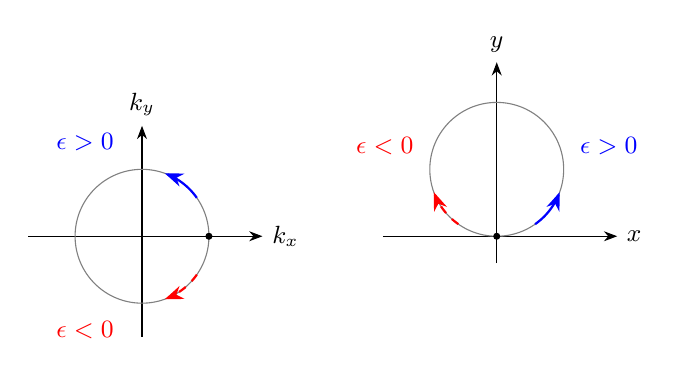
\begin{tikzpicture}[>=Stealth,font=\small,scale=0.85]
  \begin{scope}[xshift=0cm]
    \draw[->] (-1.7,0)--(1.8,0) node[right] {$k_x$};
    \draw[->] (0,-1.5)--(0,1.65) node[above] {$k_y$};
    \draw[thin,gray] (0,0) circle (1);
    \draw[->,blue,thick] plot[domain=35:70,samples=16] ({cos(\x)},{sin(\x)});
    \draw[->,red,dashed,thick] plot[domain=-35:-70,samples=16] ({cos(\x)},{sin(\x)});
    \fill (1,0) circle (1.5pt);
    \node[blue] at (-0.85,1.4) {$\epsilon>0$};
    \node[red] at (-0.85,-1.4) {$\epsilon<0$};
  \end{scope}
  \begin{scope}[xshift=5.3cm]
    \draw[->] (-1.7,0)--(1.8,0) node[right] {$x$};
    \draw[->] (0,-0.4)--(0,2.6) node[above] {$y$};
    \draw[thin,gray] (0,1) circle (1);
    \fill (0,0) circle (1.5pt);
    \draw[->,blue,thick] plot[domain=35:70,samples=16] ({sin(\x)},{1-cos(\x)});
    \draw[->,red,dashed,thick] plot[domain=35:70,samples=16] ({-sin(\x)},{1-cos(\x)});
    \node[blue,right] at (1.1,1.35) {$\epsilon>0$};
    \node[red,left] at (-1.1,1.35) {$\epsilon<0$};
  \end{scope}
\end{tikzpicture}
\caption{線形バンドの波数円と実空間円。実線の矢印は正の枝、破線の矢印は負の枝の時間発展方向を示す。}
\label{fig:linear-orbits}
\end{figure}

\end{document}
